\section*{Introduction}

GenAlg is a C library providing structures and functions implementing a Genetic Algorithm.\\ 

The genes are memorized as a VecFloat and/or VecShort. The user can defined a range of possible values for each gene. The user can define the size of the pool of entities and the size of the breeding pool. Selection, reproduction and mutation are designed to efficiently explore all the possible gene combination, and avoid local optimum. It is also possible to save and load the GenAlg.\\

It uses the \begin{ttfamily}PBErr\end{ttfamily}, \begin{ttfamily}PBMath\end{ttfamily} and \begin{ttfamily}GSet\end{ttfamily} libraries.\\

\section{Definitions}

A genetic algorithm has 3 steps. In a pool of entities it discards a given number of entities based on their ranking (given by a mean external to the algorithm). Then it replaces each of the discarded entity by a new one created from two selected entities from hte non discarded one. The newly created entity's properties are a mix of these two selected entities, plus a certain amount of random modification. The detail of the implementation in GenAlg of these 3 steps (selection, reproduction and mutation) are given below.\\

\subsection{Selection}

The non discarded entities are called 'elite' in GenAlg. The size of the pool of elite is configurable by the user. The selection of two elite entities is simply a random selection in the pool of elites. Selection of the same elite twice is allowed.\\

\subsection{Reproduction}

The reproduction step copies the genes of the elite entity into the new entity. Each gene has a probability of 50\% to be chosen in one or the other elite.\\

\subsection{Mutation}

The mutation occurs as follow. First we calculate the probability of mutation for every gene as follow: $P=\frac{rank}{nbEntity}$ where rank is the rank of the discarded entity in the pool of entities, and nbEntity is the number of entities in the pool. A gene affected by a mutation according to this probability is modified as follow. The amplitude of the mutation is equal to $1-\frac{1}{\sqrt{age+1}}$ where age is the age of the oldest elite entity used during the reproduction step for the entity. Then the new value of the gene is equals to $gene+range*amp*(rnd+delta)$ where gene is the current value of the gene, range is equal to $max_{gene}-min_{gene}$ (the difference of the maximum allowed value for this gene and its minimum value), amp is the amplitude calculated above, rnd is a random value between -0.5 and 0.5, and delta is the mutation that has been applied to this gene in the corresponding elite entity. Genes' value is kept in bounds by bouncing it on the bounds when necessary ($gene=2*bound-gene$)\\

To counteract inbreeding (the algorithm getting stuck into a local minimum), we also apply mutation to all the entities except the best one when the diversity level of the elite pool fall below a threshold (set to 0.01 by default). The diversity level is calculated as follow $\frac{1}{nbElite}\sum_{i=1}^{nbElite}\frac{||\overrightarrow{adn}(elite_i)-\overrightarrow{adn}(elite_0)||}{||\overrightarrow{bound}_{max}-\overrightarrow{bound}_{min}||*Age(elite_i)}$ where nbElite is the number of elite entities, $\overrightarrow{adn}(elite_i)$ is the genes vector of the i-th elite entity, and $\overrightarrow{bound}_{max}$ and $\overrightarrow{bound}_{min}$ are the vector of maximum and minimum values of the genes.\\ 

Some explanation: delta bias the mutation toward the direction that improved the result at previous step; in the pool of discarded entities high ranked ones tend to have few mutations and low ranked ones tend to have more mutation, this tends to cover any posibilities of evolution; entities newly entered in the elite pool tends to produce new entities near to them (in term of distance in the genes space), while older ones tend to produce more diverse new entities, thus the exploration of solution space occurs from the vicinity of newly better solutions toward larger areas; from the previous point, a good entity tends to create a lot of similar entity, which may lead to an elite pool saturated with very similar entities (inbreeding) from which the algorithm can't escape, this is prevented by the forced mutation of elites when the inbreeding level gets too high.\\

\section{Interface}

\begin{scriptsize}
\begin{ttfamily}
\verbatiminput{/home/bayashi/Coding/GenAlg/genalg.h}
\end{ttfamily}
\end{scriptsize}

\section{Code}

\subsection{genalg.c}

\begin{scriptsize}
\begin{ttfamily}
\verbatiminput{/home/bayashi/Coding/GenAlg/genalg.c}
\end{ttfamily}
\end{scriptsize}

\subsection{genalg-inline.c}

\begin{scriptsize}
\begin{ttfamily}
\verbatiminput{/home/bayashi/Coding/GenAlg/genalg-inline.c}
\end{ttfamily}
\end{scriptsize}

\section{Makefile}

\begin{scriptsize}
\begin{ttfamily}
\verbatiminput{/home/bayashi/Coding/GenAlg/Makefile}
\end{ttfamily}
\end{scriptsize}

\section{Unit tests}

\begin{scriptsize}
\begin{ttfamily}
\verbatiminput{/home/bayashi/Coding/GenAlg/main.c}
\end{ttfamily}
\end{scriptsize}

\section{Unit tests output}

\begin{scriptsize}
\begin{ttfamily}
\verbatiminput{/home/bayashi/Coding/GenAlg/unitTestRef.txt}
\end{ttfamily}
\end{scriptsize}

UnitTestGenAlgLoadSave.txt:\\
\begin{scriptsize}
\begin{ttfamily}
\verbatiminput{/home/bayashi/Coding/GenAlg/UnitTestGenAlgLoadSave.txt}
\end{ttfamily}
\end{scriptsize}

UnitTestGenAlgTest.txt:\\
\begin{scriptsize}
\begin{ttfamily}
\verbatiminput{/home/bayashi/Coding/GenAlg/UnitTestGenAlgTest.txt}
\end{ttfamily}
\end{scriptsize}

eval() of best genes over epoch:\\
\begin{center}
\begin{figure}[H]
\centering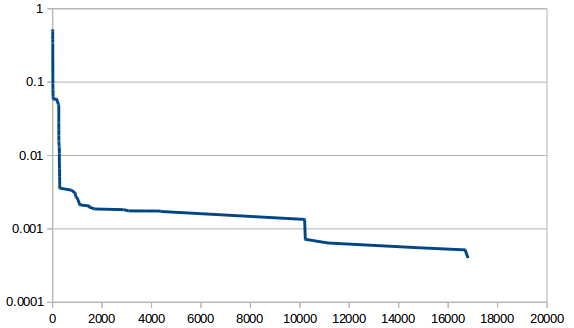
\includegraphics[width=10cm]{./eval.png}\\
\end{figure}
\end{center}

inbreeding over epoch:\\
\begin{center}
\begin{figure}[H]
\centering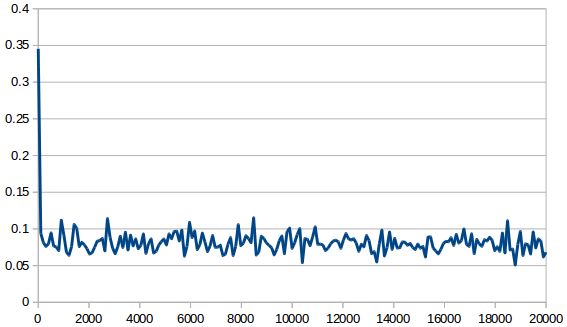
\includegraphics[width=10cm]{./inbreeding.png}\\
\end{figure}
\end{center}
\begin{center}
\begin{figure}[H]
\centering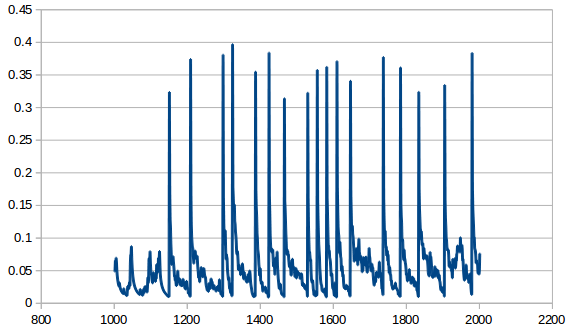
\includegraphics[width=10cm]{./inbreeding-extract.png}\\
\end{figure}
\end{center}
